\section{Desarrollo de Firmware}


El desarrollo del firmware se abordó desde varios puntos que se trabajaron en paralelo para garantizar su correcto funcionamiento. El firmware desarrollado fue estructurado considerando que el lenguaje de programación utilizado es C++, optando por la filosofía de programación orientada a objetos. Por lo tanto, se implementaron clases independientes para los diferentes módulos del sistema, como Sensórica, Control y el Receptor FlySky. Estas clases son gestionadas desde el programa principal (main), asegurando una organización modular y facilitando el mantenimiento y la escalabilidad del código. Esta metodología permite una interacción clara y definida entre los distintos componentes del sistema, asegurando que cada módulo funcione de manera autónoma pero coordinada dentro del controlador de vuelo del UAV.

\subsection{Entorno de Programación}

El firmware desarrollado para el controlador de vuelo fue escrito en C++ utilizando el framework de \textbf{Espressif}. Para el desarrollo y gestión del proyecto se empleó PlatformIO, una herramienta multiplataforma que permite programar en diferentes boards de manera eficiente y flexible. El entorno de programación utilizado fue Visual Studio Code, que ofrece una interfaz amigable y numerosas extensiones útiles para el desarrollo de proyectos embebidos. \\ \\

Inicialmente, el proyecto fue diseñado y programado para una board ESP32. Posteriormente, se migró a una ESP32-S3, una versión más reciente y avanzada de este microcontrolador. Esta migración se realizó para aprovechar las mejoras y características adicionales que ofrece la ESP32-S3, asegurando un rendimiento superior y una mayor capacidad de procesamiento para las tareas del controlador de vuelo.

\begin{comment}
    

\section{ESP32-S3}
El núcleo del sistema o \textbf{MCU} es el microcontrolador ESP32-S3 de Espressif, un System on ChipSoC (SoC) que integra funcionalidades avanzadas de Wi-Fi y Bluetooth LE, optimizado para aplicaciones de bajo consumo energético y alta eficiencia en la comunicación. Facilita la integración con una amplia variedad de sensores y actuadores a través de interfaces periféricas, utilizando protocolos estándar de la industria como I2C, UART y SPI.\cite{ESP32S3}

\vspace{10 px}
\subsection{\textbf{Descripción del Pinout del ESP32-S3}}
El pinout del ESP32-S3 es crucial para la interfaz con diversos sensores y actuadores en el controlador de vuelo. A continuación, se describen algunos pines específicos y su funcionalidad dentro del sistema: 

\begin{figure}[H]
    \centering
    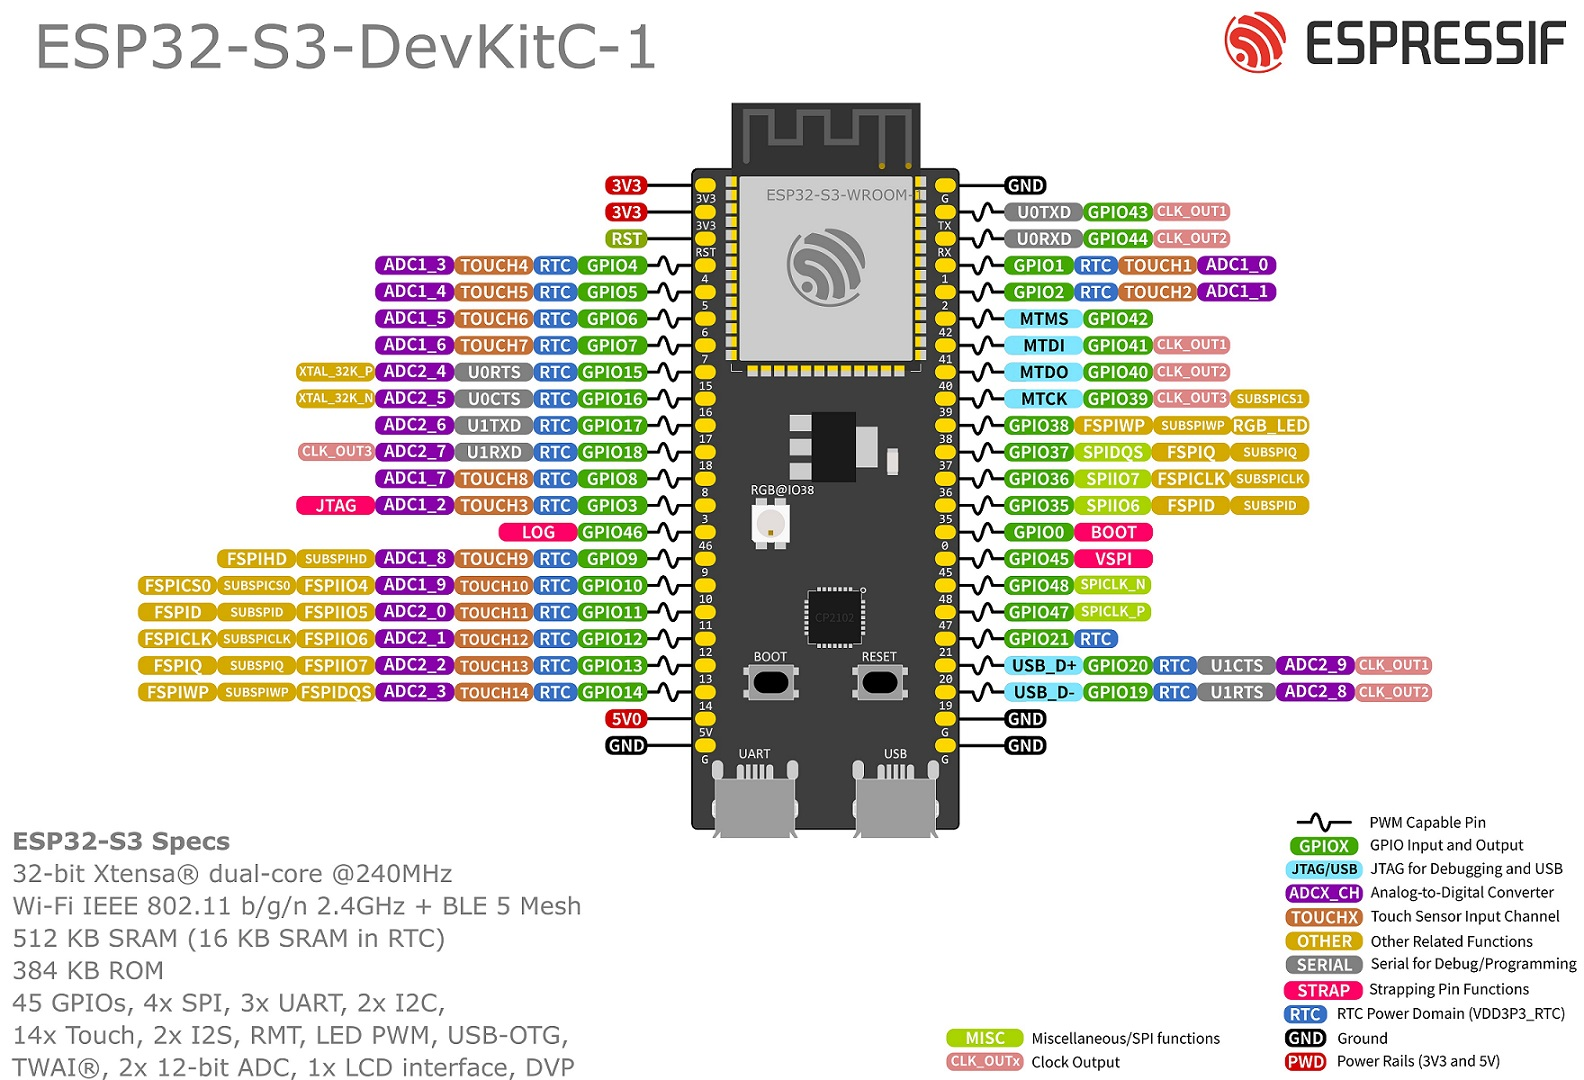
\includegraphics[width=6 in]{Imagenes/Metodologia/ESP32-S3_DevKitC-1_pinlayout_v1.1.jpg}
    \caption{Pinout del ESP32-S3 \cite{ESP32S3}}
    \label{fig:arqui_controlador}
\end{figure}





\paragraph{\textbf{Pines de Comunicación Serial (UART)}}
\begin{itemize}
    \item \textbf{GPIO1 (U0TXD)} y \textbf{GPIO3 (U0RXD)}: Estos pines son utilizados para la comunicación UART, esencial para la transmisión de datos hacia y desde el módulo GPS. La capacidad de comunicación bidireccional es fundamental para recibir datos de ubicación y enviar configuraciones al GPS.
    \item \textbf{GPIO17 (U1TXD)} y \textbf{GPIO18 (U1RXD)}: Pines alternativos para comunicación UART, utilizados para conectar dispositivos adicionales que requieran comunicación serial.\cite{ESP32S3}
\end{itemize}

\paragraph{\textbf{Pines I2C}}
\begin{itemize}
    \item \textbf{GPIO5 (SCL)} y \textbf{GPIO4 (SDA)}: Estos pines facilitan la comunicación I2C, usados principalmente para interconectar sensores como el BMP280 (sensor de presión) y el IMU. Permiten la transmisión de comandos y la recepción de datos del sensor de manera eficiente.\cite{ESP32S3}
\end{itemize}

\paragraph{\textbf{Pines de Alimentación y Control}}
\begin{itemize}
    \item \textbf{3V3 y GND}: Pines de alimentación que proveen la energía necesaria para el funcionamiento del ESP32-S3 y los periféricos conectados. Es crucial asegurar una conexión estable y de adecuada capacidad de corriente para evitar reinicios inesperados o malfuncionamiento del hardware.
    \item \textbf{EN (Enable)}: Pin utilizado para habilitar o reiniciar el microcontrolador. Un pulso bajo en este pin puede reiniciar el sistema, lo cual es útil durante el desarrollo y en situaciones de error en campo.
\end{itemize}

\paragraph{\textbf{Pines de Propósito General (GPIO)}}
\begin{itemize}
    \item \textbf{GPIO21, GPIO22, GPIO23}: Pines configurables para entrada o salida general, utilizados en este proyecto para controlar LEDs indicadores de estado, actuadores o leer señales de sensores adicionales.
\end{itemize}

\paragraph{Pines Especiales}
\begin{itemize}
    \item \textbf{GPIO0 (BOOT)}: Utilizado para entrar en el modo de programación del ESP32-S3 al inicio. Debe estar en bajo durante el reinicio para activar la carga de nuevos programas, lo que es esencial durante las fases de desarrollo y prueba.
\end{itemize}

Esta configuración de pines permite la interacción entre el microcontrolador y los distintos componentes del sistema de control de vuelo, asegurando la operatividad y la eficiencia en la gestión de los recursos y tareas asignadas.
\\ \\
\subsection{Hardware Serial}
ESP32-S3 soporta múltiples canales UART, lo que permite una comunicación serial robusta y flexible. Esta capacidad es esencial para el intercambio de datos en tiempo real entre el controlador de vuelo y otros componentes del sistema, como módulos GPS y sensores IMU, garantizando una transmisión de datos eficiente y confiable.
\\ \\
\subsection{Modo de arranque}
El modo de arranque del ESP32-S3 se configura mediante el estado de varios pines de arranque durante el reset del dispositivo. Esto proporciona una flexibilidad significativa para la carga de diferentes programas y el desarrollo de software, permitiendo que el dispositivo se adapte a diversas aplicaciones y escenarios de uso. El modo de arranque puede influir en cómo el dispositivo gestiona la seguridad del arranque y la integridad del firmware.
\\
\subsection{Carga de programa}
La carga de programas en el ESP32-S3 se realiza a través de interfaces estándar como UART o mediante el puerto USB. El entorno de desarrollo proporciona herramientas que facilitan la escritura, el debug y la carga de software, soportando lenguajes como C y Python. Esto permite a los desarrolladores programar el dispositivo con facilidad, implementar actualizaciones de firmware y realizar mantenimiento en campo.\\ \\

\subsection{Procesador y memoria}
\paragraph{\textbf{Procesador de doble núcleo}}
El procesador de \textbf{doble núcleo del ESP32-S3} opera a una frecuencia de hasta \textbf{240 MHz}, proporcionando una capacidad de procesamiento considerable para tareas múltiples y simultáneas. Esta característica es crítica para aplicaciones que requieren respuestas rápidas y procesamiento en tiempo real, como el control de vuelo en UAVs. \cite{ESP32S3}\\

\paragraph{\textbf{Memoria interna}}
El ESP32-S3 está equipado con memoria interna suficiente para gestionar las operaciones del sistema y el almacenamiento temporal de datos. La memoria interna se divide en varios bloques, incluyendo ROM para el arranque y firmware básico, y SRAM para la ejecución de programas y almacenamiento de variables durante la operación.cite{ESP32S3}\\

\paragraph{\textbf{Memoria externa}}
El microcontrolador soporta memoria externa a través de interfaces SPI, permitiendo la expansión del almacenamiento para aplicaciones que acumulan grandes volúmenes de datos, como registros de vuelo o datos sensoriales. La flexibilidad en la gestión de la memoria externa facilita la implementación de sistemas complejos y la adaptación a requerimientos específicos de almacenamiento y procesamiento.\cite{ESP32S3}\\

%end{comment}

\subsection{Verificación de Conectividad Sensores y Actuadores }
Antes de proceder con la sensórica, es fundamental realizar una verificación de los sensores y actuadores conectados al sistema. Este paso incluye un escaneo de las direcciones de los dispositivos I2C, asegurando que todos los componentes estén correctamente conectados al bus I2C. Este escaneo permite identificar qué dispositivos están presentes y si falta alguno, lo que facilita la detección de problemas de conexión antes de inicializar el programa.\\ \\

\\ \\
\subsubsection{Escaneo de direcciones I2C} \\ \\

Para determinar el correcto funcionamiento del bus I2C, se diseñó un software que detecta los dispositivos conectados al bus y cuántos hay. Este procedimiento se ejecuta cada vez que se inicia el dispositivo. A continuación, se presentan los resultados del escaneo de direcciones I2C:\\ \\

\begin{figure}[H]
    \centering
    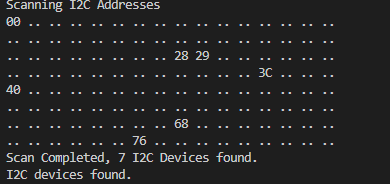
\includegraphics[width=10 cm]{Imagenes/Metodologia/I2C_scan.png}
    \caption{Escaneo I2C de los dispositivos conectados.}
    \label{fig:i2c_scan}
\end{figure}

Los dispositivos detectados en el bus I2C y sus correspondientes direcciones son:\\ \\

\begin{itemize}
    \item \textbf{0x28}: Corresponde al tubo de Pitot.
    \item \textbf{0x29}: Corresponde al sensor de orientación \textbf{BNO055}.
    \item \textbf{0x40}: Corresponde al controlador de servos PCA9685.
    \item \textbf{0x76}: Corresponde al sensor de presión barométrica BMP280.
    \item \textbf{0x68}: Corresponde al acelerómetro y giroscopio \textbf{MPU6050}.
    \item \textbf{0x00}: Corresponde a la pantalla OLED.
\end{itemize}\\ \\





\subsection{Sensorica y adquisición de datos} \\ \\

    Los sensores son uno de los componentes más críticos en el controlador de vuelo, proporcionando los datos necesarios para la navegación y el control de estabilidad del UAV. Estos incluyen dos Unidades de Medición Inerciales \textbf{IMUs} para la detección de movimiento y orientación de la aeronave, un \textbf{barómetro} para medir la presión atmosférica y la altura de la aeronave. Finalmente un módulo \textbf{GPS} para obtener la posición geográfica de la aeronave en todo momento. \\ \\


\subsubsection{ Unidades de Medición Inerciales} \\ \\


    En el tema de las Unidades de Medición Inerciales IMUs se selecciono como IMU principal al \textbf{BNO055} debido a que es un sensor de alta precisión que integra acelerómetro, giroscopio, magnetómetro y un procesador ARM Cortex-M0 para el cálculo en tiempo real de la orientación y movimiento, ofreciendo datos fiables y precisos con una frecuencia de actualización de hasta 100 Hz \cite{IMU}. En contraste, el \textbf{MPU6050}, aunque menos avanzado, es una opción económica que proporciona seis grados de libertad y capacidades decentes para la medición de movimiento y orientación gracias a su giroscopio y acelerómetro integrados. Se comunican ambos a través del protocolo de comunicación I2C y se puede programar para diferentes sensibilidades.\cite{BNO} \\ 
    
    
    
    En caso de que se produzca un fallo con el \textbf{BNO055}, el \textbf{MPU6050} serviría como un sistema de respaldo eficiente. Aunque no ofrece la misma precisión y el conjunto de características que el \textbf{BNO055}, su capacidad para proporcionar seguimiento de movimiento y datos de inclinación lo convierte en un sustituto confiable que puede mantener la funcionalidad del sistema hasta cierto nivel hasta que se resuelva el problema principal. \\ 

    La comparación entre las especificaciones del sensor \textbf{BNO055} y el sensor \textbf{MPU6050} revela diferencias significativas en sus capacidades de procesamiento de datos y aplicaciones. El \textbf{BNO055}, como se detalla en el Cuadro \ref{tab:bno055_specs}, ofrece cálculos internos que proporcionan la orientación del dispositivo en diferentes formatos, incluidos grados, radianes y cuaterniones. Esto significa que el \textbf{BNO055} entrega directamente datos de orientación tridimensional, vector de velocidad angular, vector de aceleración, vector de fuerza del campo magnético y temperatura, sin necesidad de procesamiento adicional. Este enfoque integrado facilita su uso en aplicaciones donde se requiere una rápida interpretación y utilización de los datos de movimiento.  \\ 
    
    Por otro lado, el sensor \textbf{MPU6050}, según el Cuadro \ref{tab:mpu6050_specs}, requiere un postprocesamiento de la aceleración angular en cada uno de los ejes del dispositivo para obtener la orientación. Mientras que el \textbf{MPU6050} proporciona datos de giroscopio y acelerómetro en bruto, junto con soporte para filtros y funciones programables, el cálculo de la orientación en grados, radianes o cuaterniones debe realizarse externamente. Esto implica un esfuerzo adicional en el procesamiento de datos para lograr el mismo nivel de interpretación inmediata que ofrece el \textbf{BNO055}. \\ 
    
    En resumen, mientras que el \textbf{BNO055} simplifica la integración y el uso con su capacidad de cálculo interno de orientación, el \textbf{MPU6050} requiere un procesamiento posterior de los datos para obtener resultados similares, lo que puede ser una consideración importante en el diseño y la implementación de sistemas que dependen de la precisión y rapidez de los datos de orientación.

    
\paragraph{\textbf{\textbf{BNO055}}}

    \begin{table}[h]
\centering
\caption{Especificaciones del Sensor \textbf{BNO055}}
\label{tab:bno055_specs}
\begin{tabular}{|l|l|}
\hline
\textbf{Característica} & \textbf{Descripción} \\ \hline
Orientación Absoluta (Vector Euler, 100Hz) & Datos de orientación tridimensional basados en una esfera de 360° \\ \hline
Orientación Absoluta (Quaternión, 100Hz) & Salida de cuaternión de cuatro puntos para manipulación precisa de datos \\ \hline
Vector de Velocidad Angular (100Hz) & Tres ejes de 'velocidad de rotación' en rad/s \\ \hline
Vector de Aceleración (100Hz) & Tres ejes de aceleración (gravedad + movimiento lineal) en m/s\textsuperscript{2} \\ \hline
Vector de Fuerza del Campo Magnético (20Hz) & Tres ejes de detección de campo magnético en micro Tesla (uT) \\ \hline
Vector de Aceleración Lineal (100Hz) & Tres ejes de datos de aceleración lineal (aceleración menos gravedad) en m/s\textsuperscript{2} \\ \hline
Vector de Gravedad (100Hz) & Tres ejes de aceleración gravitacional (menos cualquier movimiento) en m/s\textsuperscript{2} \\ \hline
Temperatura (1Hz) & Temperatura ambiente en grados Celsius \\ \hline
\end{tabular}
\end{table}

\begin{table}[H]
\centering
\caption{Especificaciones del Sensor \textbf{MPU6050}}
\label{tab:mpu6050_specs}
\begin{tabular}{|l|l|}
\hline
\textbf{Característica} & \textbf{Descripción} \\ \hline
Giroscopio & Salida digital en ejes X, Y, Z con escalas de ±250, ±500, ±1000, y ±2000°/sec \\ \hline
Acelerómetro & Salida digital de 3 ejes con escalas de ±2g, ±4g, ±8g, y ±16g \\ \hline
Voltaje de Trabajo & 2.375-3.46V \\ \hline
Voltaje de Lógica I2C & 1.71V a VDD \\ \hline
Interface Serial & I2C \\ \hline
ADC & 16 bits para giroscopio y acelerómetro \\ \hline
Procesador de Movimiento & DMP integrado para procesamiento de movimiento en 3D y algoritmo de reconocimiento de gestos \\ \hline
Filtros & Filtros pasa bajo programables \\ \hline
Interrupciones Programables & Soporta funciones como reconocimiento de gestos, detección de golpe y movimiento \\ \hline
\end{tabular}
\end{table}
\\ \\
\paragraph{\large \textbf{ Marcos de Referencia para la Medición de Ángulos en el Controlador de Vuelo}} \\ \\

Inicialmente, se estableció el marco de referencia de los ángulos que va a medir el controlador con respecto al marco de referencia del UAV. Los ejes ilustrados representan las orientaciones críticas: yaw (giro alrededor del eje vertical), pitch (inclinación hacia adelante o hacia atrás) y roll (rotación sobre el eje longitudinal) \ref{fig:movimientos_inerciales}. Estos ángulos son fundamentales para el control de la orientación del UAV, y el controlador de vuelo está diseñado para recopilar y procesar datos sobre cada uno de estos ejes, permitiendo así ajustes precisos en tiempo real para mantener la estabilidad del dispositivo.

\begin{figure}[H]
    \centering
    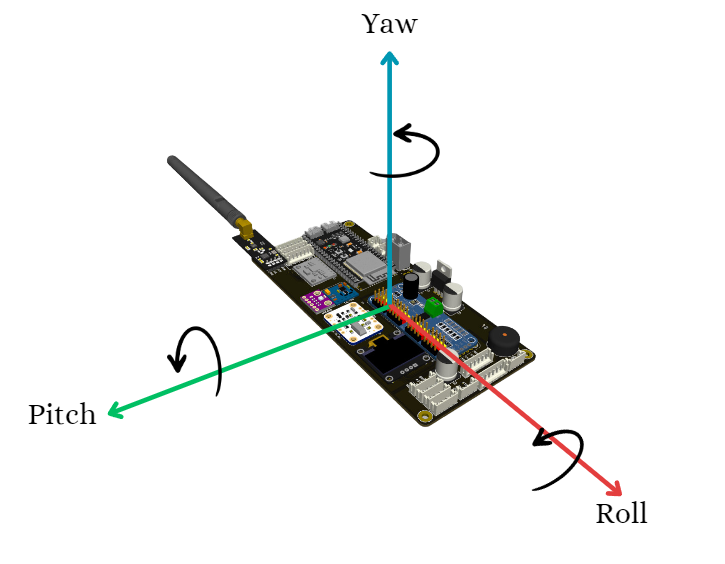
\includegraphics[width=0.8\textwidth]{Imagenes/Metodologia/pcb_yaw_pitch_roll.png}
    \caption{Movimientos Inerciales Yaw, Pitch y Roll en el controlador de vuelo}
    \label{fig:movimientos_inerciales}
\end{figure}
\\ \\
\paragraph{\large \textbf{Filtrado y recopilación de datos de movimientos inerciales}}
\\ \\

Para este apartado, se leyeron y procesaron datos tomados del sensor \textbf{MPU6050}. Se realizó un algoritmo en el que se aplican filtros de Kalman para estimar los ángulos de orientación del dispositivo (Roll, Pitch, Yaw) a partir de las mediciones del sensor. Esto con el objetivo de mejorar la precisión de estas estimaciones al reducir el ruido y combinar de manera óptima ambas fuentes de datos. \\ 

El filtro de Kalman es un enfoque matemático que se utiliza ampliamente en aplicaciones de control y navegación para estimar el estado de sistemas dinámicos a partir de mediciones ruidosas. Este algoritmo se basa en dos fases principales: predicción y actualización. Estas se utilizan iterativamente para mejorar la estimación del estado del sistema con cada nueva medición.
\\ \\
\subparagraph{\textbf{\large Fase de Predicción}} \\ \\

En la fase de predicción, el filtro de Kalman utiliza un modelo del sistema para predecir el próximo estado, basándose en el estado estimado actual y en el conocimiento de cómo evoluciona el sistema con el tiempo. Esta predicción también incluye una estimación de la incertidumbre (o error) asociada con el estado predicho. La incertidumbre se modela como una matriz de covarianza, que cuantifica la confianza en la predicción del estado. Para esto se tiene que: \\

\[
\hat{x}_{k|k-1} = A\hat{x}_{k-1|k-1} + B u_k
\]
\[
P_{k|k-1} = A P_{k-1|k-1} A^T + Q
\]
\\
En donde:

\\
\begin{itemize}
    \item $\hat{x}_{k|k-1}$ es la estimación del estado en el tiempo $k$, dada la información hasta el tiempo $k-1$.
    \item $A$ es la matriz del modelo de transición del estado.
    \item $\hat{x}_{k-1|k-1}$ es la estimación del estado en el tiempo $k-1$, dada toda la información hasta el tiempo $k-1$.
    \item $B$ es la matriz del modelo de control.
    \item $u_k$ es el vector de control en el tiempo $k$.
    \item $P_{k|k-1}$ es la covarianza del error de predicción en el tiempo $k$.
    \item $Q$ es la covarianza del ruido del proceso.
\end{itemize}
\\ \\
En esta fase de predicción, se actualizará el ángulo de Roll basado en la velocidad angular previa, ajustada por el sesgo estimado, y el paso de tiempo. Además, se actualizan las matrices de covarianza de error para reflejar la nueva incertidumbre después de la predicción.

\subparagraph{\textbf{\large Fase de Actualización}}

En la fase de actualización, se ajusta la estimación del estado con base en la nueva medición:

\[
K_k = P_{k|k-1} H^T (H P_{k|k-1} H^T + R)^{-1}
\]
\[
\hat{x}_{k|k} = \hat{x}_{k|k-1} + K_k (z_k - H \hat{x}_{k|k-1})
\]
\[
P_{k|k} = (I - K_k H) P_{k|k-1}
\]

En donde:
\begin{itemize}
    \item $K_k$ es la ganancia de Kalman en el tiempo $k$.
    \item $H$ es la matriz del modelo de observación.
    \item $R$ es la covarianza del ruido de observación.
    \item $z_k$ es la medición real en el tiempo $k$.
    \item $I$ es la matriz identidad, con dimensiones adecuadas para la operación.
\end{itemize}
\\ \\
En esta fase de actualización, se calcula la discrepancia entre la estimación del ángulo a partir del acelerómetro y la predicción del ángulo de Roll. Además, se calculan las ganancias de Kalman, que determinan cómo se combinan la predicción y la medición para obtener una nueva estimación. Por otro lado, se actualizan el ángulo estimado de Roll y el sesgo utilizando las ganancias de Kalman. Por último, se ajustan las matrices de covarianza de error para reflejar la disminución en la incertidumbre después de la actualización. \\

Estas ecuaciones se aplican de forma iterativa para cada nueva medición, mejorando así la estimación del estado del sistema a lo largo del tiempo. \\

En las Figuras  \ref{fig:pitch} y \ref{fig:roll}, se muestran las gráficas obtenidas al implementar este algoritmo. En estas gráficas podemos ver la diferencia de los datos obtenidos mediante el \textbf{MPU6050} antes del proceso de filtrado (\textit{Raw}) y después de aplicar el filtro de Kalman (\textit{Filtered}).
\\ \\
\begin{figure}[H]
    \centering
    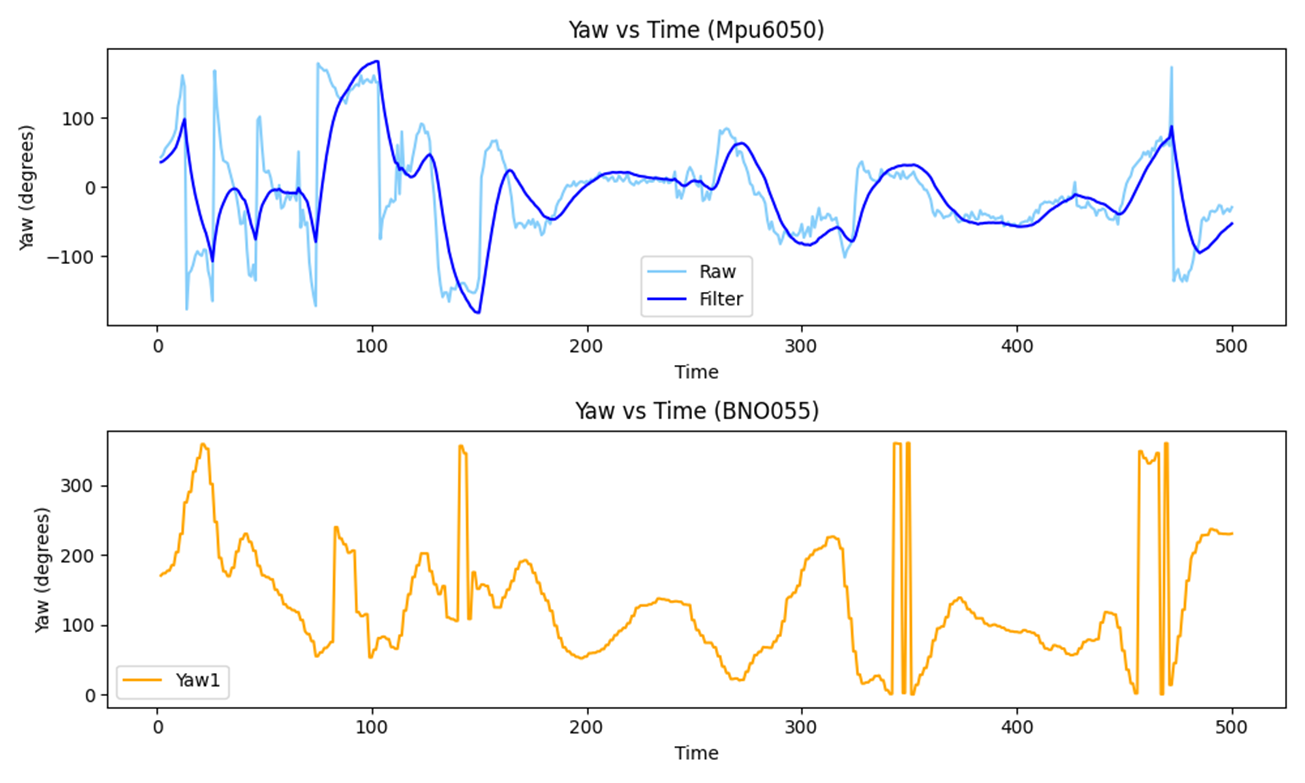
\includegraphics[width=0.8\textwidth]{Imagenes/Metodologia/Angulos_Giro_pitch_Mpu6050_BNO055.png}
    \caption{Ángulos de Giro Pitch obtenidos con \textbf{MPU6050} y \textbf{BNO055}.}
    \label{fig:pitch}
\end{figure}

\begin{figure}[H]
    \centering
    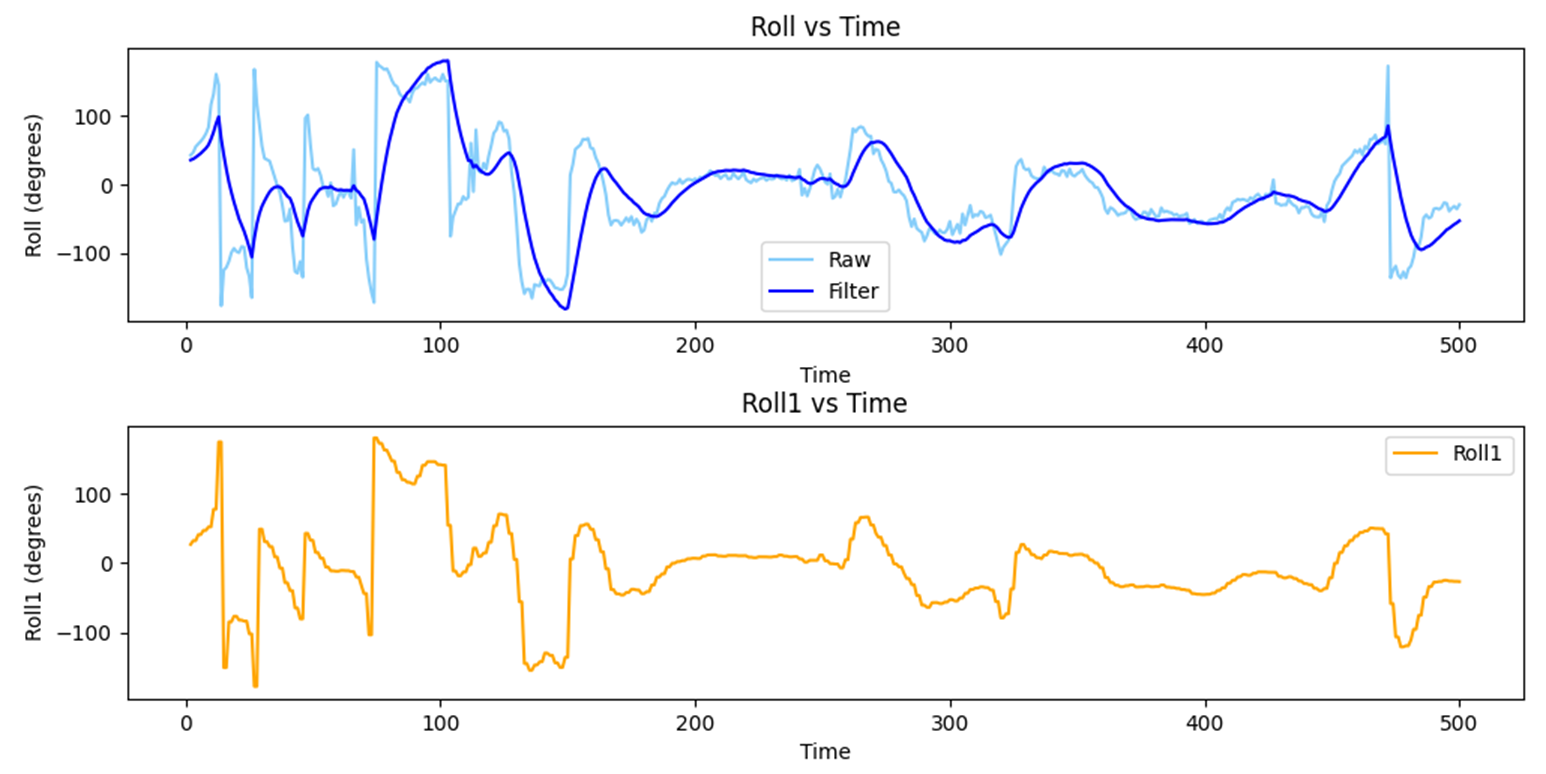
\includegraphics[width=0.8\textwidth]{Imagenes/Metodologia/Angulos_Giro_roll_Mpu6050_BNO055.png}
    \caption{Ángulos de Giro Roll obtenidos con \textbf{MPU6050} y \textbf{BNO055}.}
    \label{fig:roll}
\end{figure}

\begin{figure}[H]
    \centering
    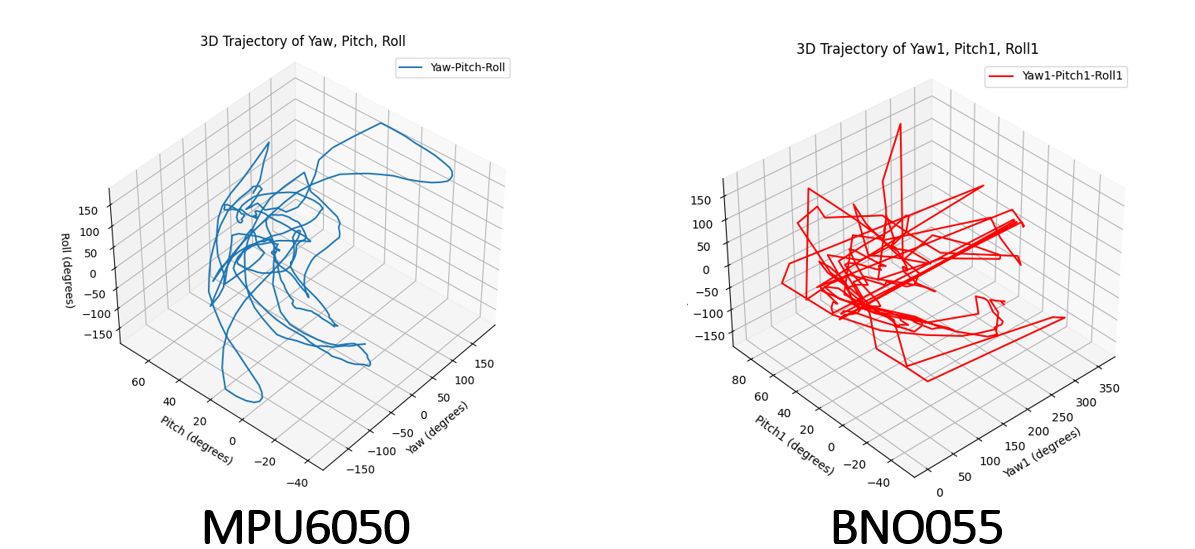
\includegraphics[width=0.8\textwidth]{Imagenes/Metodologia/Angulos_Giro_Mpu6050_BNO055.png}
    \caption{Ángulos de Giro \textbf{MPU6050} y \textbf{BNO055}.}
    \label{fig:3d_trajectory}
\end{figure}

\\ \\
\paragraph{ \large \textbf{Protocolo de Inicialización y Recepción de Datos del BNO055}}

\\ \\
\begin{enumerate}
    \item \textbf{Detección del Sensor}:
    \begin{itemize}
        \item El sensor \textbf{BNO055} se inicializa y se intenta establecer comunicación en la dirección I2C predeterminada. Si no se detecta el sensor, se muestra un mensaje de error en el monitor serie.
    \end{itemize}

    \item \textbf{Calibración del Sensor}:
    \begin{itemize}
        \item Se entra en un bucle de calibración donde se verifica continuamente el estado de calibración del sensor. Durante este proceso, se muestra el estado de calibración en una pantalla OLED.
    \end{itemize}

    \item \textbf{Contador de 5 Segundos}:
    \begin{itemize}
        \item Después de la calibración, se muestra un contador de 5 segundos en la pantalla OLED, permitiendo que el usuario coloque el dispositivo en una posición de referencia estable.
    \end{itemize}

    \item \textbf{Cálculo y Visualización de los Offsets}:
    \begin{itemize}
        \item Se calculan los offsets de los ángulos (roll, pitch y yaw) en la posición de referencia y se muestran en la pantalla OLED.
    \end{itemize}
\end{enumerate}
\\ \\
\paragraph{\large Recepción de Datos del \textbf{BNO055}}
\\ \\
\begin{enumerate}
    \item \textbf{Lectura de Datos de Orientación}:
    \begin{itemize}
        \item Se leen los valores de orientación (yaw, pitch y roll) del sensor y se ajustan estos valores restando los offsets calculados previamente.
    \end{itemize}

    \item \textbf{Lectura de Datos del Acelerómetro}:
    \begin{itemize}
        \item Se leen los valores de aceleración en los ejes X, Y y Z.
    \end{itemize}

    \item \textbf{Lectura de Datos del Magnetómetro}:
    \begin{itemize}
        \item Se leen los valores del campo magnético en los ejes X, Y y Z.
    \end{itemize}

    \item \textbf{Cálculo del Valor de la Brújula}:
    \begin{itemize}
        \item Se calcula el valor del heading utilizando los datos del magnetómetro y luego se aplica un filtro de Media Exponencialmente Ponderada (EMA) para suavizar el valor del heading.
    \end{itemize}
\end{enumerate}



\paragraph{\large  \textbf{Cálculo del Heading}}
\\ \\
El heading (rumbo) se calcula utilizando los componentes X e Y del campo magnético:
\\ \\
\[
\text{heading\_rad} = \text{atan2}(my, mx)
\]

\[
\text{heading\_deg} = \text{heading\_rad} \times \frac{180.0}{\pi}
\]
\\ \\
Si el valor calculado del heading es negativo, se ajusta sumándole 360 grados para obtener un valor positivo:
\\ \\
\[
\text{if} \ (\text{heading\_deg} < 0) \ \text{then} \ \text{heading\_deg} += 360
\]

\paragraph{\large Suavizado del Heading con EMA}
\\ \\
Para reducir la oscilación en los valores de heading, se aplica un filtro de Media Exponencialmente Ponderada (EMA). La fórmula para actualizar el valor suavizado es:
\\ \\
\[
\text{smoothedHeading} = \alpha \times \text{newHeading} + (1 - \alpha) \times \text{oldHeading}
\]

Donde \(\alpha\) es el factor de suavizado. Para manejar la discontinuidad alrededor de 360 grados, se ajusta la diferencia de los valores de heading:

\[
\text{diff} = \text{newHeading} - \text{oldHeading}
\]

\[
\text{if} \ (\text{diff} > 180) \ \text{then} \ \text{oldHeading} += 360
\]

\[
\text{else if} \ (\text{diff} < -180) \ \text{then} \ \text{oldHeading} -= 360
\]

Finalmente, se ajusta el valor suavizado para mantenerse dentro del rango de 0 a 360 grados:
\\ \\
\[
\text{if} \ (\text{smoothedHeading} \geq 360) \ \text{then} \ \text{smoothedHeading} -= 360
\]

\[
\text{else if} \ (\text{smoothedHeading} < 0) \ \text{then} \ \text{smoothedHeading} += 360
\]
\\ 
Este método asegura que los valores de heading se mantengan dentro del rango de 0 a 360 grados y se suavicen adecuadamente, reduciendo las fluctuaciones en la señal.
\\ \\
\subsubsection{Barómetro, Altímetro y Termómetro}
\\ \\
Un barómetro es un instrumento capaz de medir la presión atmosférica, proporcionando datos esenciales para la predicción del tiempo y la altitud. En el contexto de sensores modernos, como el \textbf{BMP280}, estas funcionalidades se amplían significativamente. El BMP280 no solo actúa como un barómetro, sino que también integra un altímetro y un termómetro. Esto permite obtener medidas precisas de presión, altitud y temperatura en un solo dispositivo compacto. La capacidad de medir la presión atmosférica es crucial para determinar la altitud en aplicaciones de navegación y control de un UAV de ala fija, mientras que la medición de la temperatura ayuda a saber la temperatura del controlador de vuelo.\\ \\
\paragraph{\large  \textbf{Inicialización del BMP280}}\\ \\

Al iniciar el sensor BMP280, se configura la presión atmosférica de referencia para \textbf{Bogotá} en \textbf{1028} hPa. Luego, se lee la altura inicial basada en esta referencia. Si la inicialización del sensor falla, se imprime un mensaje de error en el monitor serial. El proceso de inicialización garantiza que las lecturas de altura sean precisas y consistentes con la altitud específica de Bogotá.
\\ \\
\paragraph{\large  \textbf{Aplicación del EMA (Exponential Moving Average)}}\\ \\

Para suavizar las lecturas de presión atmosférica, altura y temperatura interna del dispositivo, se está aplicando un algoritmo de Media Móvil Exponencial (EMA). Este algoritmo es útil para reducir el ruido en los datos y proporcionar valores más estables y representativos. El EMA calcula el promedio ponderado de los datos recientes, donde los datos más recientes tienen un peso mayor en el cálculo del promedio. Esto se realiza para cada una de las mediciones (presión, altura y temperatura) obtenidas del BMP280. \\

La fórmula utilizada para el cálculo del EMA es la siguiente:
\\ \\
\[
\text{EMA} = (\alpha \cdot \text{currentReading}) + ((1 - \alpha) \cdot \text{previousEMA})
\]
\\ \\
Donde:
\begin{itemize}
    \item \text{currentReading} es la lectura actual del sensor.
    \item \text{previousEMA} es el valor del EMA anterior.
    \item $\alpha$ es el factor de suavizado, un valor entre 0 y 1 que determina el peso de la lectura actual en el cálculo del EMA.
\end{itemize}
\\ \\
\paragraph{\large  \textbf{Proceso de Lectura de Datos}}
\\ \\
\begin{enumerate}
    \item \textbf{Presión Atmosférica}: Se obtiene directamente del sensor y se aplica el EMA para suavizar las lecturas.
    \item \textbf{Altura}: Se calcula en función de la presión atmosférica y se ajusta utilizando la altura inicial leída durante la inicialización. También se aplica el EMA para obtener una lectura más estable.
    \item \textbf{Temperatura Interna}: Se mide directamente desde el BMP280 y se procesa mediante el EMA para reducir el ruido en las lecturas.
\end{enumerate}\\ \\



\subsubsection{Sistema de Posicionamiento Global (GPS)}\\ \\


Para asegurar una alta fiabilidad y precisión en la ubicación del UAV, se seleccionó el \textbf{GPS M10Q-5883}. Este dispositivo integra el módulo GNSS SAM-M10Q-00B de u-blox, capaz de recibir simultáneamente señales de cuatro constelaciones \textbf{satelitales: GPS, GLONASS, Galileo y BeiDou}.\cite{GPS} Esta capacidad multiconstelación amplía significativamente la cobertura y mejora la disponibilidad de la señal en condiciones adversas, como en entornos urbanos densos o áreas con obstrucciones. Además, el módulo GNSS SAM-M10Q-00B emplea tecnología avanzada que optimiza la sensibilidad y reduce el tiempo de adquisición de señal, garantizando así una ubicación precisa y dinámica incluso en escenarios complicados. Utilizando el protocolo de comunicaciones UART, este sistema transmite datos de posición de manera precisa y confiable, asegurando que el UAV pueda navegar y operar de forma óptima en diversas condiciones. \\ \\

\paragraph{\large  \textbf{Proceso de Inicialización del GPS}}
Para inicializar el GPS es necesario establecer la comunicación serial con el dispositivo. Esto se logra utilizando el siguiente código, que configura los pines TX2 y RX2 para la comunicación serial: \\ \\
\begin{lstlisting}[language=C++]
const int TX2 = 11;
const int RX2 = 10;
Serial2.begin(9600, SERIAL_8N1, RX2, TX2);
\end{lstlisting}

\\ \\

Una vez que el GPS está conectado y se inicializa la comunicación serial, el dispositivo se encenderá con una luz verde. Es importante situar el GPS en un lugar con cielo abierto, ya que tardará unos minutos en obtener la recepción de las señales de los satélites. Una vez que el módulo recibe la señal de los satélites, comenzará a titilar, indicando que se ha establecido correctamente la comunicación con el satélite. \\

Para contrastar y validar que los valores recibidos por el GPS eran correctos, se utilizó la aplicación GnssLogger de Google (véase la Figura \ref{fig:gpsGnss}). En esta prueba, se compararon los datos obtenidos por el GPS con los proporcionados por la red WLS (Wireless Location Service) y el GPS del celular. La prueba se realizó en la terraza del quinto piso del edificio Mario Laserna. Se encontró que todos los datos de ubicación se encontraban dentro de un radio de aproximadamente 6 metros, lo que confirma la precisión de los datos recibidos. \\ 

\begin{figure}[H]
    \centering
    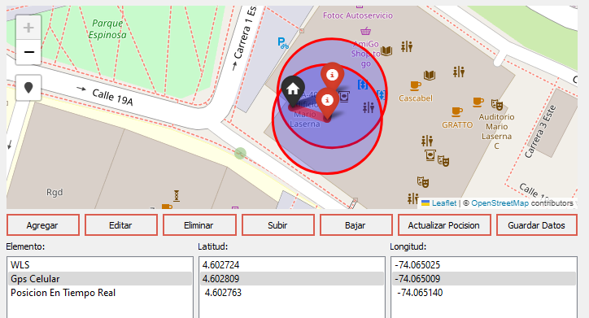
\includegraphics[width=10 cm]{Imagenes/Firmware/GPS.png}
    \caption{Validación de la precisión del GPS utilizando GnssLogger.}
    \label{fig:gpsGnss}
\end{figure}



%\subsection{Pantalla Oled 1,3}

\\ \\
\subsection{Recopilación y Almacenamiento de Datos}
\\ \\
En el ámbito de las aeronaves, la recopilación y el almacenamiento de datos juegan un papel crucial. Este dispositivo es esencial, ya que permite registrar la información histórica del vuelo, proporcionando un registro detallado de todos los eventos y parámetros operativos. Actúa como una "caja negra" que almacena datos vitales que pueden ser utilizados para análisis post-vuelo, mantenimiento preventivo, y en el desafortunado caso de una eventualidad, para la investigación de incidentes. La capacidad de recopilar y almacenar datos de manera confiable asegura que toda la información relevante del vuelo esté disponible para su revisión.
\subsubsection{SD TF}

El módulo lector de microSD, también conocido como SD (Secure Digital), es un componente esencial en el dispositivo. Este módulo permite guardar la información y los datos generados por los sensores y los cálculos realizados por la \textbf{ESP32-S3}. La microSD funciona mediante un sistema de archivos que permite almacenar y recuperar datos de forma eficiente y confiable. Al inicializar la comunicación con el módulo a través de la \textbf{ESP32-S3}, se pueden escribir y leer datos en la tarjeta microSD. La información recopilada se almacenará en formato CSV (Comma-Separated Values), lo que facilita la organización y el análisis posterior de los datos.
\begin{figure}[H]
    \centering
    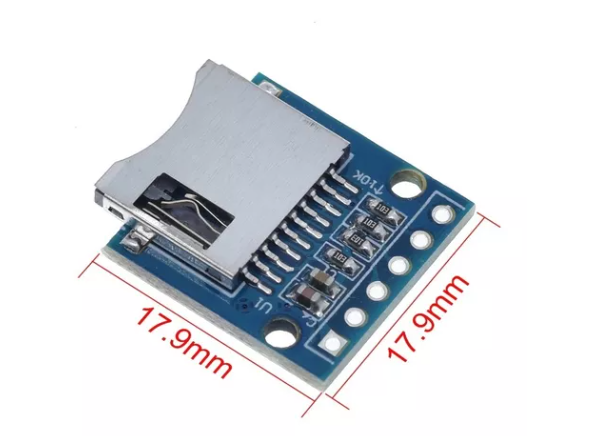
\includegraphics[width=2 in]{Imagenes/Metodologia/SD.png}
    \caption{Lector de tarjetas MicroSD}
    \label{fig:microSD}
\end{figure}
\textbf{Especificaciones Técnicas}
\begin{itemize}
    \item Modelo: Módulo lector SD TF
    \item Interfaz: SPI
    \item Voltaje de operación: 3.3V - 5V
    \item  Compatibilidad: Tarjetas microSD
\end{itemize} \\ \\
\subsubsection{Conexión y Configuración} \\\\

El módulo lector SD se comunica con el ESP32-S3 a través del protocolo SPI. A continuación, se detallan las conexiones entre el módulo lector SD y el ESP32-S3: \\ \\

\begin{itemize}
    \item MISO (Master In Slave Out): Conectado al pin MISO del ESP32-S3   \textbf{GPIO 37}
    \item MOSI (Master Out Slave In): Conectado al pin MOSI del ESP32-S3  \textbf{GPIO 35}
    \item SCK (Serial Clock): Conectado al pin SCK del ESP32-S3        \textbf{GPIO 36}
    \item CS (Chip Select): Conectado a un pin GPIO del ESP32-S3       \textbf{GPIO 38}
\end{itemize} \\ \\




\subsection{Telecomunicaciones}

En el apartado de telecomunicaciones es importante resaltar la presencia de dos componentes principales que son cruciales para el control y monitoreo del UAV. \\ 

El primer componente es el módulo de radiofrecuencia, el cual se encarga de recibir la información del operador de vuelo. Este módulo permite que la aeronave responda a los comandos enviados por el operador, facilitando el control y la maniobrabilidad del UAV. La comunicación por radiofrecuencia es esencial para asegurar que los comandos se transmitan de manera eficiente y sin retrasos, permitiendo una respuesta inmediata del UAV a las instrucciones del operador.\\ 

El segundo componente es el módulo de telemetría, que tiene la capacidad de recibir información del UAV en tiempo real. Este módulo proporciona datos vitales sobre el estado y la posición de la aeronave, incluyendo parámetros como la altitud, velocidad, orientación y otros datos críticos de vuelo. La telemetría en tiempo real es fundamental para el monitoreo continuo del UAV.\\ 
\subsubsection{Módulo de radiofrecuencia Fly-Sky FS-IA6B}

En el apartado de radiofrecuencia, se utilizo el transmisor y receptor FS-i6 de la empresa FlySky el cual es un controlador de radio digital de 6 canales diseñado para ofrecer un control preciso y fiable para diversas aplicaciones de modelismo, como drones, aviones, helicópteros y coches RC. Este transmisor utiliza la tecnología AFHDS 2A (Automatic Frequency Hopping Digital System) para asegurar una comunicación sin interferencias y una alta inmunidad al ruido. \cite{flysky}

\textbf{Características Principales:}
\begin{itemize}
    \item \textbf{Frecuencia:} 2.4 GHz AFHDS 2A.
    \item \textbf{Canales:} 6 canales programables.
    \item \textbf{Pantalla LCD:} Proporciona una interfaz gráfica para la configuración y el monitoreo en tiempo real.\cite{19}
    \item \textbf{Rango de Operación:} Hasta 1 km en condiciones óptimas.\cite{19}
    \item \textbf{Compatibilidad:} Compatible con diversos receptores FlySky que soportan AFHDS 2A.\cite{flysky}
    \item \textbf{Funciones:} Incluye funciones avanzadas como mezcla de canales, configuración de servos, límite de puntos finales, y modos de vuelo.   \cite{flysky}
\end{itemize}

Para interconectar este sistema de radio control con el controlador de vuelo, se procedió a realizar un análisis de cómo sería la comunicación del receptor con el dispositivo (véase \ref{fig:radio_arqui}). Se descubrió que cada uno de los 6 canales del dispositivo envía una señal \textbf{PWM}, por lo que, si se procesa esta información con la \textbf{ESP32-S3} y se decodifica esta señal, es posible transcribir este ancho de pulso en valores para que la \textbf{PCA9685} pueda mover los servos al valor deseado.


\begin{figure}[H]
    \centering
    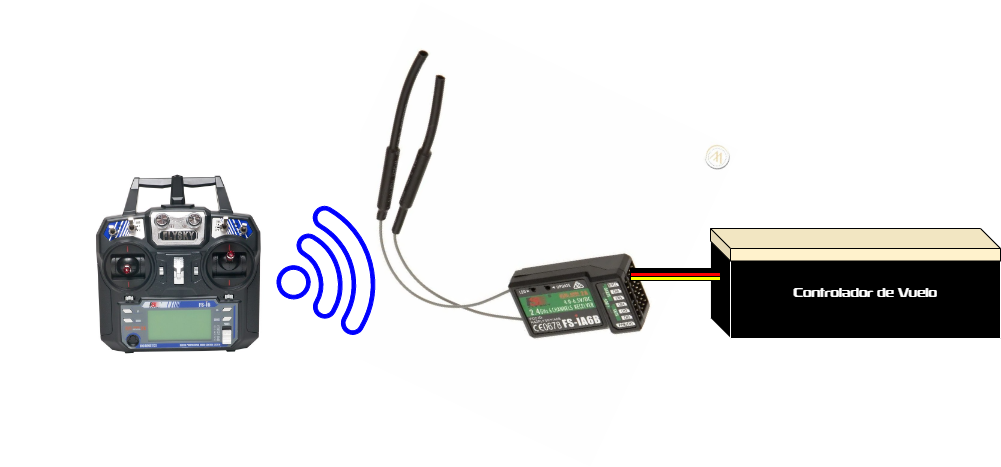
\includegraphics[width=6 in]{Imagenes/Metodologia/Radio Control.drawio.png}
    \caption{Conexión del Radio Control con el Controlador de Vuelo}
    \label{fig:radio_arqui}
\end{figure}

Este sistema se realizó de esta forma ya que es posible decodificar la información del transmisor  \textbf{Fly-Sky FS-IA6B} y poder efectuar una respuesta en los actuadores de la aeronave. Es importante destacar el hecho de al estar leyendo la información y posteriormente  enviando esta información a los \textbf{servos} se genera un pequeño \textbf{delay} que debe tenerse en cuenta al momento de operar la aeronave.

\vspace{5 px}
\paragraph{\textbf{Proceso de Decodificación}}
\vspace{5 px}
Para decodificar las señales PWM, se utiliza la función \texttt{pulseIn} del microcontrolador, que mide la duración del pulso en microsegundos. Esta duración se mapea a un rango de valores especificado mediante la función \texttt{map}.
\vspace{5 px}
\paragraph{\textbf{Medición del Pulso}}
\vspace{5 px}
La función \texttt{pulseIn} mide el tiempo durante el cual la señal es alta (nivel lógico alto). Esta duración, \( t \), se expresa en microsegundos (\(\mu\)s). El rango típico de estas duraciones para las señales PWM del receptor FLYSKY-I6B es:

\begin{equation*}
t \in [1007 \, \mu s, 1999 \, \mu s]
\end{equation*}
\vspace{5 px}
\paragraph{\textbf{Mapeo de la Señal}}
\vspace{5 px}
Para convertir la duración del pulso a un valor utilizable, se utiliza la función \texttt{map}. La función mapea el rango de entrada \([1007, 1999]\) a un rango de salida especificado por los parámetros \texttt{minLimit} y \texttt{maxLimit}. Estos parámetros descritos anteriormente hacen referencia al valor máximo y mínimo al que pueden llegar cada uno de los servomotores de la aeronave, típicamente este valor es \textbf{-30°} y \textbf{30°} con respecto al valor de referencia inicial del servo, el cual generalmente es de \textbf{90°}. A continuación se muestra la ecuación de mapeo:


\begin{equation*}
y = \frac{(\texttt{maxLimit} - \texttt{minLimit})}{(1999 - 1007)} \cdot (t - 1007) + \texttt{minLimit}
\end{equation*}
\vspace{5 px}
\paragraph{\textbf{Condiciones de Valor por Defecto}}
\vspace{5 px}
Si la duración del pulso \( t \) es menor que 100 $\mu$s, se asume que la señal es inválida, y se devuelve un valor por defecto, \texttt{defaultValue}.
\vspace{5 px}
\paragraph{\textbf{Lectura de Interruptores}}
\vspace{5 px}
Para leer el estado de un interruptor, se convierte la señal PWM del canal correspondiente a un valor booleano (verdadero o falso). Este proceso implica mapear la señal a un rango de 0 a 100 y determinar si el valor resultante es mayor que 50. La ecuación de mapeo en este caso es:

\begin{equation}
z = \frac{(100 - 0)}{(1999 - 1007)} \cdot (t - 1007) + 0
\end{equation}

El resultado se evalúa para determinar el estado del interruptor:

\begin{equation}
\text{estado} = 
\begin{cases} 
\text{verdadero} & \text{si } z > 50 \\
\text{falso} & \text{si } z \leq 50 
\end{cases}
\end{equation}

A continuación se muestra un esquema (\ref{fig:decodificador_transmisor}) del transmisor FLYSKY-I6B y los valores decodificados de cada uno de los seis canales. Nótese que el \textbf{canal 1} hace referencia al movimiento de \textbf{roll}, el \textbf{canal 2} a \textbf{pitch} y el \textbf{canal 4} a \textbf{yaw} de la aeronave, controlando cada uno un servomotor que representa un movimiento particular de esta. El \textbf{canal 3} se encarga de controlar el suministro de combustible al motor. Finalmente, los canales \textbf{5 y 6} son interruptores.


\begin{figure}[H]
    \centering
    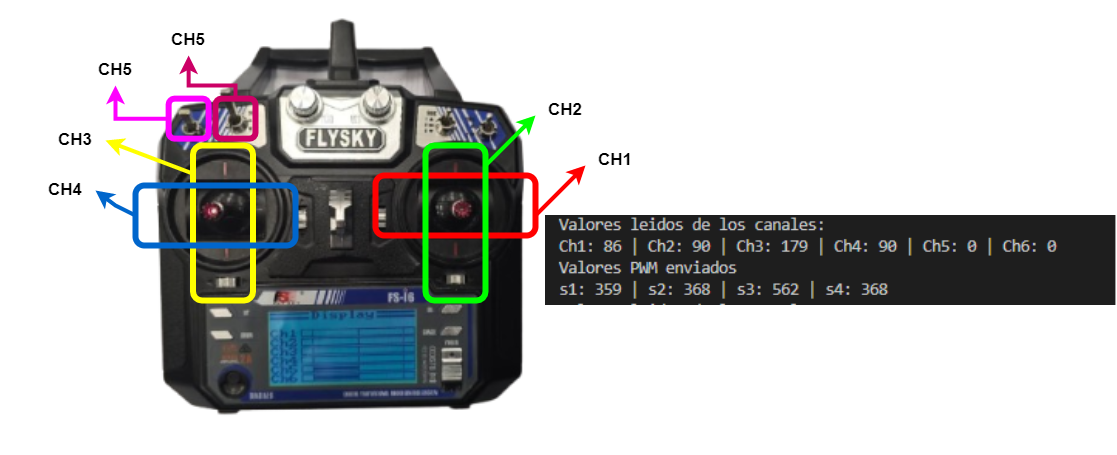
\includegraphics[width=6 in]{Imagenes/Metodologia/Diagrama Receptor.png}
    \caption{Diagrama Transmisor y decodificado de Señales PWM}
    \label{fig:decodificador_transmisor}
\end{figure}



\subsection{Telemetría}





\subsubsection{Módulo nRF24L01}\\ \\

El módulo nRF24L01 es un transceptor inalámbrico que opera en la banda de 2.4 GHz, una frecuencia comúnmente utilizada para comunicaciones de corto alcance debido a su equilibrio entre velocidad de transmisión y penetración de obstáculos. Este módulo es conocido por su bajo consumo de energía y su capacidad para manejar comunicaciones de hasta 2 Mbps.\\ 

Una de las limitaciones del nRF24L01 es su capacidad para manejar paquetes de datos de hasta 32 bits. Esto significa que los datos transmitidos deben ser empaquetados para evitar la pérdida o corrupción de la información.

\subsubsection{Estación en Tierra }\\ \\

La estación en tierra es un circuito igual que el controlador de vuelo que permite la transmisión y recepción de datos entre la aeronave y el equipo en tierra. Esta comunicación se realiza utilizando el módulo nRF24L01, previamente descrito. \\


La estación en tierra recibe los datos transmitidos por el controlador de vuelo, una vez interpretados, envía un mensaje de confirmación de recepción al controlador de vuelo. Este proceso bidireccional asegura que los datos de telemetría sean correctamente. \\

El funcionamiento de la comunicación se puede observar en la figura \ref{fig:estacion en tierra}, donde se muestra el flujo de mensajes entre la estación en tierra y el controlador de vuelo: \\ \\ 

\begin{itemize}
    \item \textbf{Transmisión:} El controlador de vuelo envía datos a la estación en tierra codificados.
    \item \textbf{Recepción:} La estación en tierra recibe los datos y los decodifica.
    \item \textbf{Mensaje de Verificación:} La estación en tierra envía un mensaje de verificación de recepción.
    \item \textbf{Confirmación:} El controlador de vuelo recibe la confirmación de que los datos fueron recibidos.
\end{itemize} \\ \\ 

Este ciclo continuo de transmisión y verificación es esencial para mantener la integridad de los datos y garantizar que cualquier ajuste necesario durante el vuelo se base en información precisa y actualizada.\\ \\ 
\begin{figure}[H]
    \centering
    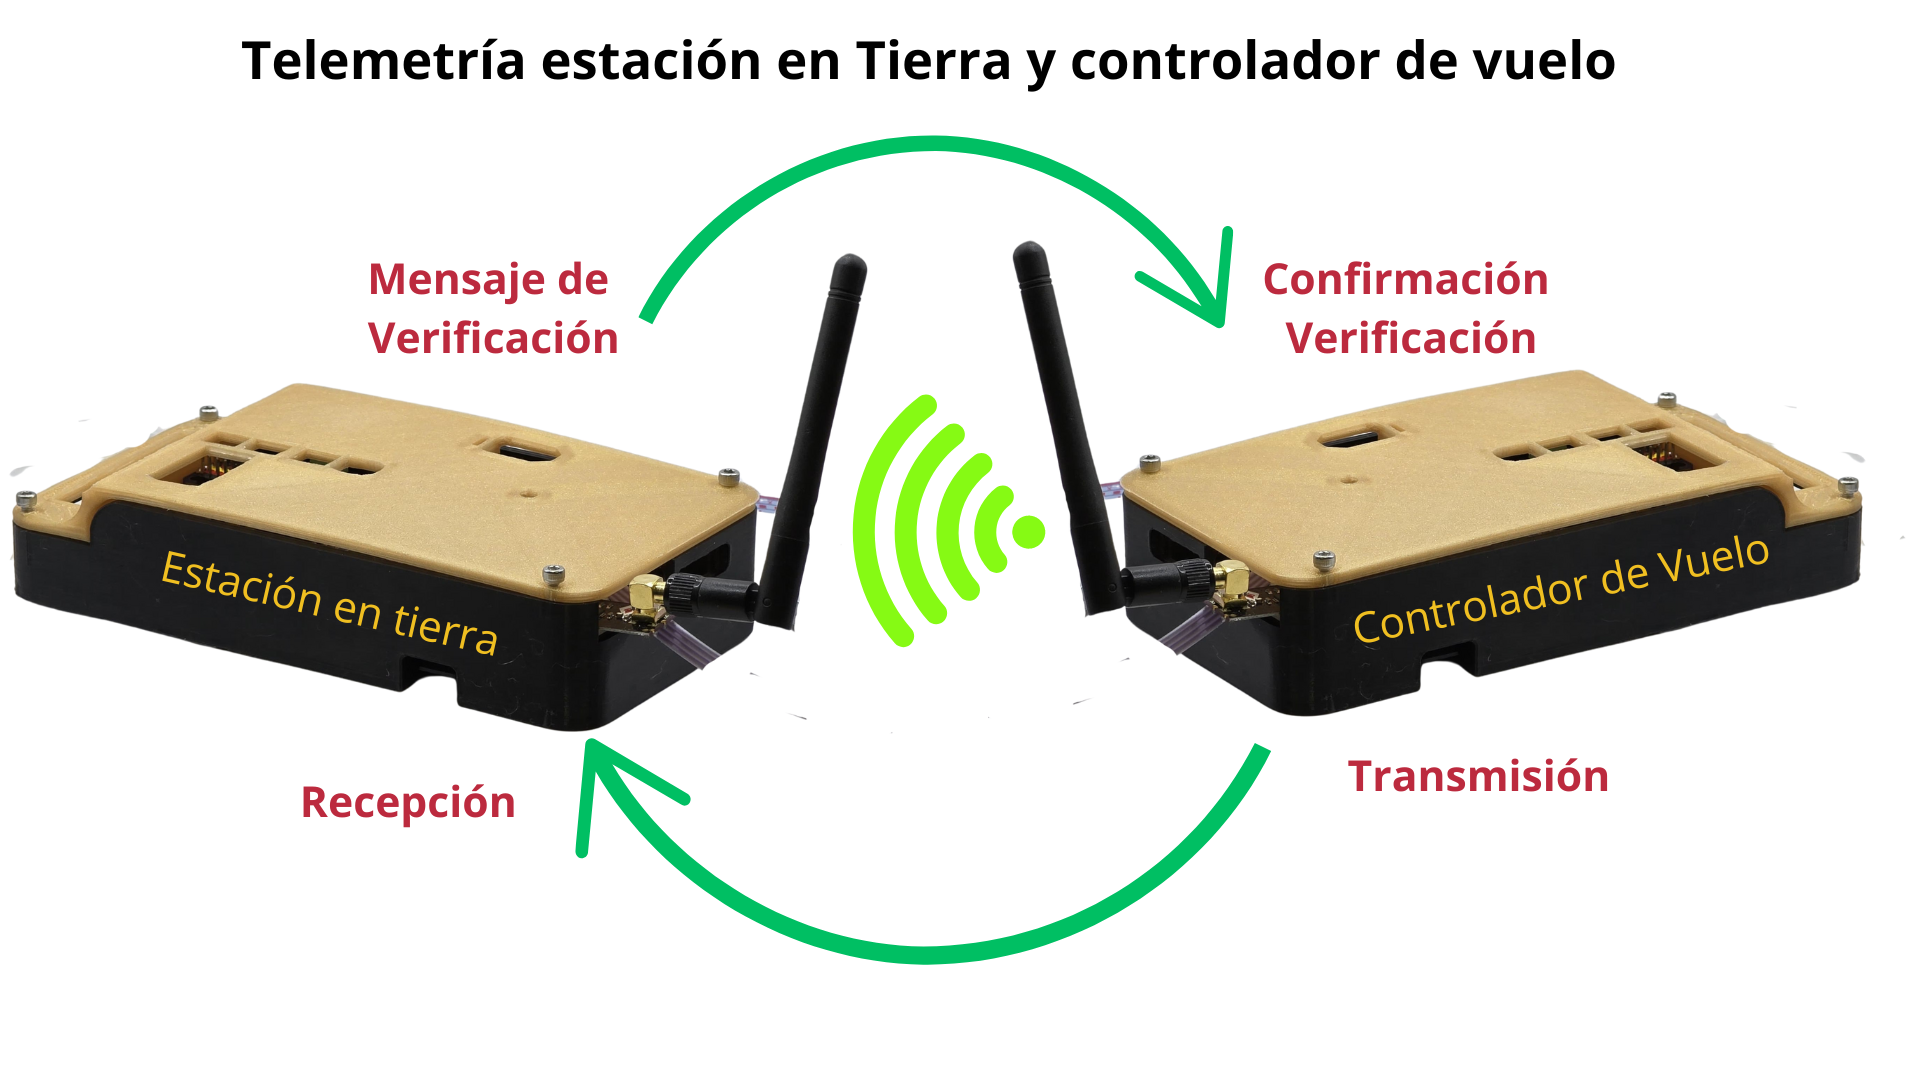
\includegraphics[width=\textwidth]{Imagenes/Metodologia/estacion en tierra.png}
    \caption{Conexión del Controlador de Vuelo y la estación en Tierra}
    \label{fig:estacion en tierra}
\end{figure} \\ \\ 



\subsubsection{Arquitectura General del Firmware Controlador de Vuelo y la Estación de Control en Tierra} \\  \\ 


La figura \ref{fig:diag-codigo } representa la arquitectura general del controlador de vuelo y la estación de control en tierra, detallando los protocolos de inicialización y las principales tareas realizadas por cada sistema. A continuación se presenta una explicación general de cada sección:\\ \\ 

\subsection{Controlador de Vuelo}\\  \\ 

\begin{itemize}
    \item \textbf{Protocolo de Inicialización}
    \begin{itemize}
        \item \textbf{Escaneo e Inicialización de Dispositivos I2C}: El sistema escanea e inicializa todos los dispositivos I2C conectados al controlador de vuelo.
        \item \textbf{Inicialización del Protocolo SPI y Creación del Archivo de Datos}: Se inicializa el protocolo SPI y se crea un archivo de datos para almacenar los datos de vuelo.
    \end{itemize}
    \\ \\ 
    \item \textbf{Bucle Principal (Mientras Está Encendido)}
    \begin{itemize}
        \item \textbf{Lectura de Sensores y GPS, Actualización de Variables Globales y Pantalla OLED}: El controlador de vuelo lee datos de varios sensores y del módulo GPS, actualiza las variables globales y la pantalla OLED.
        \item \textbf{Lectura de Canales del Receptor}: El sistema lee las entradas de los canales del receptor, que contienen los comandos de control de la estación de control en tierra o del operador.
        \item \textbf{Escritura de Datos en la MicroSD}: Los datos de vuelo se escriben en una tarjeta MicroSD para su registro y análisis posterior.
        \item \textbf{Envío de Datos (Telemetría)}: Los datos de telemetría comprimidos en 32 bits se envían a la estación de control en tierra.
    \end{itemize}
    \\ \\ 
    \item \textbf{Tarea: Escritura y Movimiento de Actuadores}
    \begin{itemize}
        \item \textbf{Determinación del Modo de Operación Basado en Comandos y Datos de Vuelo}: El controlador de vuelo determina el modo de operación del UAV basado en los comandos de entrada y los datos de vuelo actuales.
        \item \textbf{Mover Actuadores}: El sistema envía comandos a los actuadores para controlar los movimientos del UAV.
    \end{itemize}
\end{itemize}
\\  \\ 
\subsection{Estación de Control en Tierra}

\begin{itemize}
    \item \textbf{Protocolo de Inicialización}
    \begin{itemize}
        \item \textbf{Escaneo e Inicialización de Dispositivos I2C}: Similar al controlador de vuelo, la estación de control en tierra escanea e inicializa todos los dispositivos I2C conectados.
        \item \textbf{Inicialización del Protocolo SPI y Creación del Archivo de Datos}: Se inicializa el protocolo SPI y se crea un archivo de datos para almacenar los datos recibidos.
    \end{itemize}
    \\  \\ 
    \item \textbf{Bucle Principal (Mientras Está Encendido)}
    \begin{itemize}
        \item \textbf{Lectura de Información de Radio}: La estación de control en tierra lee los datos recibidos vía radio desde el controlador de vuelo.
        \item \textbf{Decodificación de la Información}: Los datos recibidos se decodifican para su procesamiento.
        \item \textbf{Escritura de Datos en Serial}: Los datos decodificados se escriben en la interfaz serial para su monitoreo en tiempo real o procesamiento adicional.
        \item \textbf{Escritura de Datos en la MicroSD}: Los datos recibidos y decodificados también se registran en una tarjeta MicroSD para su análisis posterior.
    \end{itemize}
\end{itemize}
\begin{figure}[H]
    \centering
    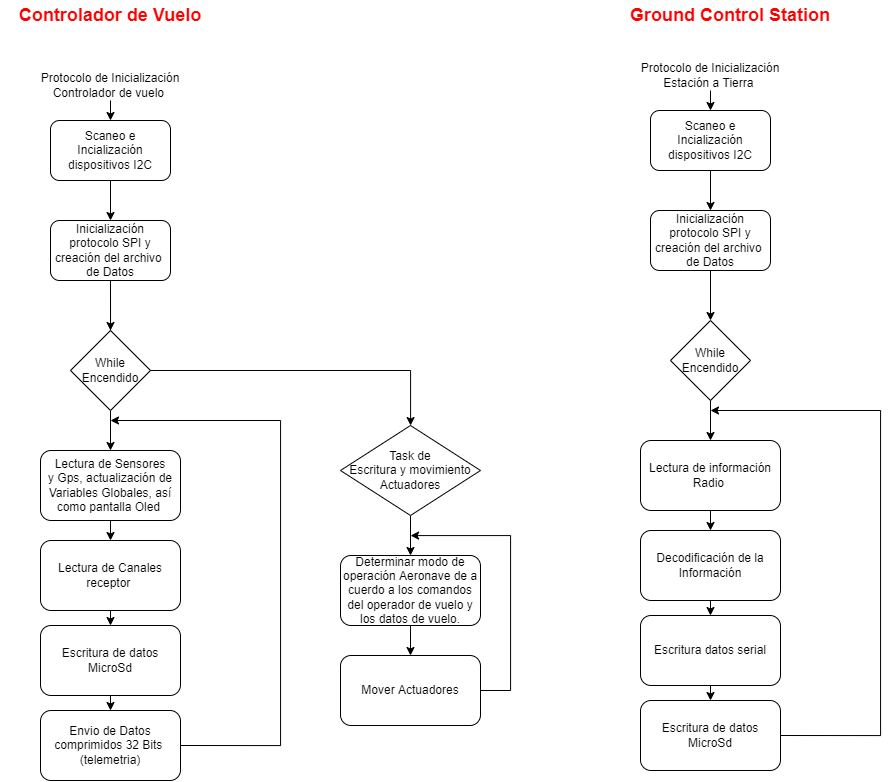
\includegraphics[width=\textwidth]{Imagenes/Interfaz/diagrama general de codigo.png}
    \caption{Diagrama general de funcionamiento Controlador y estación a Tierra }
    \label{fig:diag-codigo }
\end{figure} \\ \\




\subsection{Actuadores} \\ \\


En términos de actuadores, se trabajará con servomotores, ya que son los encargados de mover las superficies de control de la aeronave, incluyendo los alerones, timón de cola, elevadores y el sistema de propulsión eléctrico o de gasolina. \\ 

Para manejar estos distintos actuadores, se seleccionó el módulo \textbf{PCA9685} debido a su capacidad de controlar hasta 16 servomotores o actuadores simultáneamente mediante señales \textbf{PWM}. Este módulo ofrece una gestión precisa y eficiente de los componentes mecánicos de la aeronave. La elección del \textbf{PCA9685} permite una optimización del diseño y la funcionalidad del UAV, facilitando la implementación de sistemas de control complejos con una sola placa. Esto reduce la necesidad de múltiples controladores y simplifica la arquitectura del sistema. \\ \\

\subsubsection{Funcionamiento}

A la hora de leer los valores del radiotransmisor FlySky, es importante recordar que estamos mapeando la señal que devuelve en un valor angular, lo que permite al controlador determinar el ángulo al que debe fijar el servomotor. Para mover los servomotores, se debe convertir ese ángulo en un ancho de pulso PWM válido. El proceso se describe en el siguiente código: \\ 


\begin{lstlisting}[language=C++, caption=Conversión de ángulo a ancho de pulso PWM]
#define MIN_PULSE_WIDTH 600
#define MAX_PULSE_WIDTH 2600

int ReguladorServos::pulseWidth(int angle)
{
    // Función que convierte un ángulo entre 0 y 180 a un ancho de pulso (dato que leen los servos)
    int pulse_wide, analog_value;
    pulse_wide = map(angle, 0, 180, MIN_PULSE_WIDTH, MAX_PULSE_WIDTH);
    analog_value = int(float(pulse_wide) / 1000000 * FREQUENCY * 4096);
    return analog_value;
}
\end{lstlisting}

Definición de los límites del ancho de pulso:\\ 

\begin{itemize}
\item \texttt{#define MIN\_PULSE\_WIDTH 600}: Define el ancho de pulso mínimo en microsegundos.
\item \texttt{#define MAX\_PULSE\_WIDTH 2600}: Define el ancho de pulso máximo en microsegundos.
\end{itemize}

Función de conversión de ángulo a ancho de pulso:\\ 

Definición de los límites del ancho de pulso:\\

\begin{itemize}
\item \texttt{\#define MIN\_PULSE\_WIDTH 600}: Define el ancho de pulso mínimo en microsegundos.
\item \texttt{\#define MAX\_PULSE\_WIDTH 2600}: Define el ancho de pulso máximo en microsegundos.
\end{itemize}

Función de conversión de ángulo a ancho de pulso:\\

\begin{itemize}
\item La función \texttt{pulseWidth(int angle)} toma un ángulo como parámetro, que debe estar en el rango de 0 a 180 grados.
\item Se utiliza la función \texttt{map()} para convertir el ángulo en un ancho de pulso proporcional entre los valores mínimos y máximos definidos.
\item La conversión del ancho de pulso a un valor analógico adecuado para el servomotor se realiza mediante el cálculo: \texttt{analog\_value = int(float(pulse\_wide) / 1000000 * FREQUENCY * 4096);}.
\item La función devuelve este valor analógico, que representa el ancho de pulso PWM requerido para mover el servomotor al ángulo deseado.
\end{itemize}
\\ \\
Este proceso asegura que los ángulos mapeados desde la señal del radiotransmisor se conviertan correctamente en pulsos PWM que los servomotores puedan interpretar. \\ \\




\subsubsection{Movimiento Superficies de Control} \\ \\

Una vez interpretadas las señales del radiocontrol por el receptor y decodificados los ángulos deseados por el operador de vuelo, se asignan valores de movimiento a los servomotores correspondientes a las superficies de control de la aeronave. El canal 1 del receptor controla los alerones, ilustrados en la figura \ref{fig:mov-Superficies } en color morado, que manejan el roll (balanceo lateral). El canal 2 controla los elevadores , en color negro, encargados del pitch (inclinación longitudinal). El canal 3 está conectado al acelerador, regulando la potencia del motor, mientras que el canal 4 controla el timón de cola para el yaw (giro horizontal), en color verde.
\\ \\
\begin{figure}[H]
    \centering
    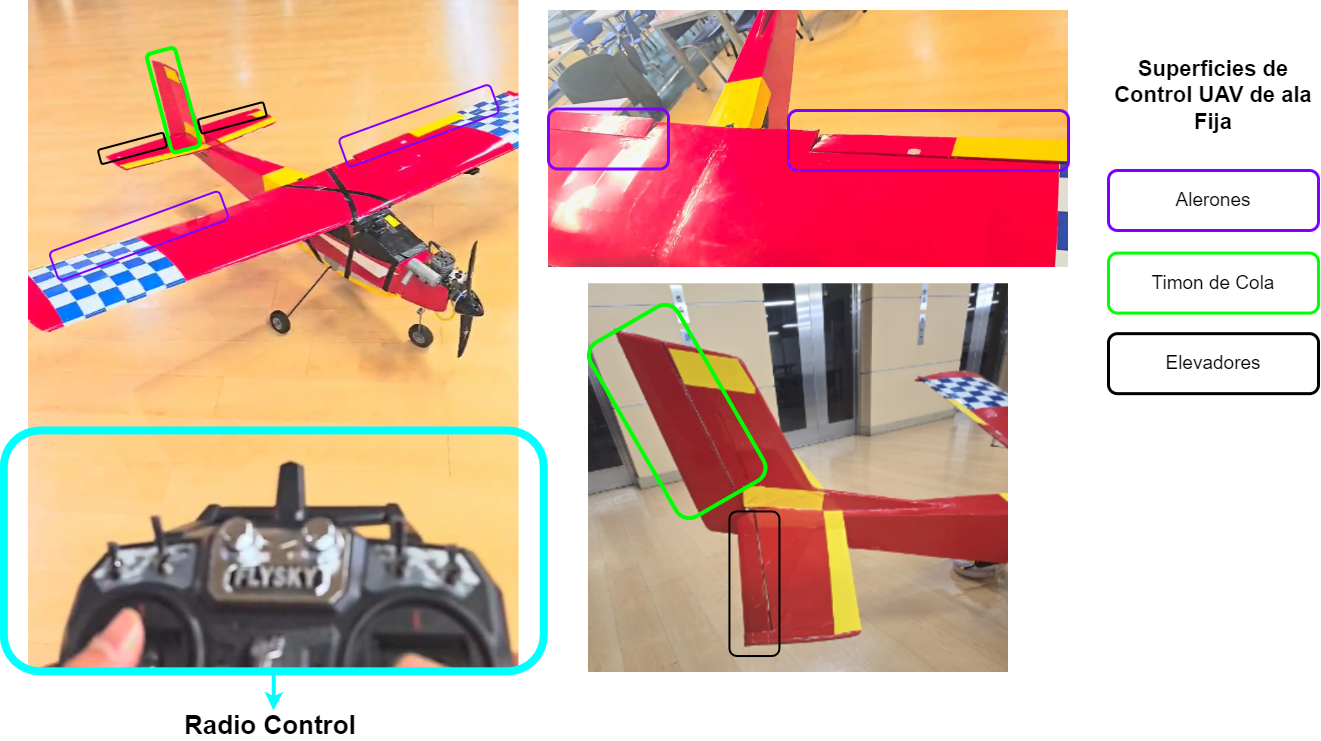
\includegraphics[width=\textwidth]{Imagenes/Firmware/Superficies de Control.png}
    \caption{Movimiento general Superficies de Control }
    \label{fig:mov-Superficies }
\end{figure} \\ \\

\\ \\
\subsection{Control} \\ \\

Para el control básico de la aeronave se estableció el siguiente modelo, en el que el operador de vuelo proporciona una señal de referencia para orientar la aeronave. Esta señal de referencia es un valor angular que indica la posición deseada. Este diagrama de PID está simplificado, ya que cada superficie de control tiene su propio PID para alcanzar la señal de referencia (véase imagen \ref{fig:pid1 }). Seguidamente, el procesador interpreta la señal de referencia que el operador de vuelo desea establecer y mueve la superficie de control correspondiente a cada señal dada por el operador. Este sistema tiene en cuenta las perturbaciones ambientales y se retroalimenta con los valores obtenidos por las unidades de movimiento inerciales (IMUs).


\begin{figure}[H]
    \centering
    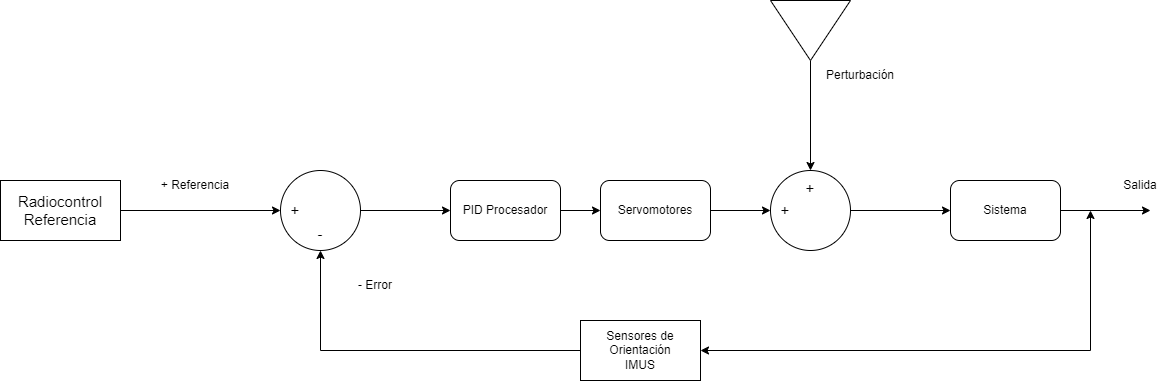
\includegraphics[width=\textwidth]{Imagenes/Firmware/PID basico.png}
    \caption{PID básico Aeronave }
    \label{fig:pid1 }
\end{figure} \\ \\

\subsubsection{Modos de Operación} \\ \\
\begin{itemize}
    \item \textbf{Modo de Vuelo de Autoestabilización:} Este es el modo de operación por defecto. En este modo, si el operador de vuelo no proporciona ninguna señal de referencia, por ejemplo, si el valor de referencia del roll es 0, el UAV de ala fija moverá los alerones para autoestabilizarse y alcanzar este valor de referencia. Este mismo principio se aplica a los ángulos de yaw y pitch, asegurando que la aeronave mantenga su orientación estable.
\\ \\
    \item \textbf{Modo de Operación Fly-by-Wire:} En este modo, el operador de vuelo establece un ángulo de referencia específico para la orientación de la aeronave. Este modo de operación se activa al encender el switch del canal 5. En este modo, el comportamiento del transmisor del radiocontrol es diferente: en lugar de enviar una señal para que un servomotor gire a un ángulo deseado, el operador envía un ángulo de referencia al que desea que esté orientada la aeronave. Los valores de los ángulos están limitados a: \\ \\

\textbf{Roll:} -25° a 25°, puesto que es el ángulo de banqueo máximo permitido para un vehículo aéreo no tripulado. \\ \\
\textbf{Pitch:}-20° a 20°, puesto que es el ángulo de elevación en el que se evita la perdida de sustentación "stall".
\end{itemize}




\subsection{Indicadores Adicionales}
\subsubsection{Dispositivo de visualización}
El sistema de control del UAV incluye un dispositivo de visualización que muestra en tiempo real indicadores cruciales como brújula, temperatura, pitch, roll, altitud, yaw, latitud y longitud. Esto permite al operador verificar el funcionamiento adecuado del UAV durante las pruebas de vuelo, asegurando que los parámetros críticos se mantengan dentro de los límites operativos. El dispositivo facilita el monitoreo continuo, la detección rápida de problemas y la validación de que todos los sistemas responden correctamente.
\begin{figure}[H]
    \centering
    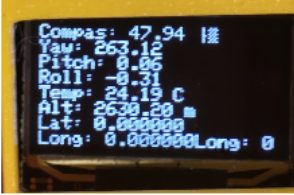
\includegraphics[width=\textwidth]{Imagenes/Firmware/Pantalla oled.png}
    \caption{PID básico Aeronave }
    \label{fig:mov-Superficies }
\end{figure} \\ \\


\subsubsection{Buzzer}

Un \textbf{Buzzer} o \textbf{zumbador} es un componente que se utiliza para emitir señales acústicas. En este caso, se utiliza para proporcionar alertas auditivas en diferentes situaciones. Como lo son la emisión de sonido para informar que el dispositivo se ha inicializado o que se ha conectado el GPS u otros módulos, también puede proporcionar alertas en caso tal de que la batería se este descargando.
\vspace{5 px}
El \textbf{Buzzer} se conecta al \textbf{ESP32-S3} a través de Un pin \textbf{GPIO}, particularmente al \textbf{GPIO-46}  configurado como salida digital. Cuando el microcontrolador envía una señal de alto nivel, el \textbf{Buzzer} emite un sonido en particular alertando al usuario del estado general del sistema.
\vspace{5 px}


\end{comment}


